% !TeX program = xelatex
\documentclass[11pt,a4paper]{ctexart}

\usepackage[margin=2.25cm]{geometry}
\usepackage{amsmath,amssymb,amsfonts}
\usepackage{graphicx}
\usepackage{subcaption}
\usepackage{float}
\usepackage{booktabs}
\usepackage{caption}
\usepackage{hyperref}
\usepackage[section]{placeins}
\usepackage{setspace}
\usepackage{indentfirst}

\hypersetup{colorlinks=true,linkcolor=black,citecolor=black,urlcolor=blue}
\graphicspath{{./}{results/figures/}{../results/figures/}}
\setstretch{1.08}
\setlength{\parindent}{2\ccwd}
\setlength{\parskip}{0pt}
\captionsetup{font=small,labelfont=bf,skip=4pt}
\captionsetup[sub]{font=small,skip=2pt}
\setlength{\abovedisplayskip}{0.65em}
\setlength{\belowdisplayskip}{0.65em}
\setlength{\textfloatsep}{0.9em plus 0.2em minus 0.15em}
\setlength{\floatsep}{0.8em plus 0.2em minus 0.15em}
\setlength{\intextsep}{0.8em plus 0.2em minus 0.15em}
\setcounter{topnumber}{2}
\renewcommand{\topfraction}{0.92}
\renewcommand{\textfraction}{0.06}
\renewcommand{\floatpagefraction}{0.82}
\ctexset{section={afterindent=true},subsection={afterindent=true}}
\raggedbottom

\title{带时间惩罚双载荷网格配送问题的 LNS 方法}
\author{赵瑞泽}
\date{2026.5}

\begin{document}
\maketitle

\begin{abstract}
\indent 本文研究含障碍网格上的双载荷配送问题。配送员从仓库出发，每趟最多服务两个目标并返回仓库，目标函数由总距离和加权迟到时间构成。针对目标数增大后小邻域方法难以同时修正错误配对与服务顺序的问题，本文提出基于大邻域搜索（LNS）的求解方法，用有序配对排列表示方案，并结合多类破坏、后悔插入修复、局部强化和概率接受机制。实验与 EDD 贪心、最近邻贪心、匹配 EDD、局部搜索和模拟退火比较。结果表明：固定迭代预算下，LNS 通常能得到更低目标值；统一 $300$ ms 时间预算下，LNS 因重构开销较大，在短时 anytime 表现上不如模拟退火和局部搜索。代码见 \url{https://github.com/Passly0616/LNS-Paper}。
\end{abstract}

\indent\textbf{关键词：} 大邻域搜索；双载荷配送；网格路径规划；时间惩罚；组合优化

\section{引言}

\indent 仓储机器人、校园配送和室内物流常可抽象为含障碍的二维网格配送问题。若配送员每趟最多服务两个目标，则方案不仅要决定路径，还要决定目标配对、趟次顺序和趟内访问顺序；再加入期望送达时间后，最短距离方案往往不再最优。

\indent 当目标数 $k$ 增大时，错误配对和错误服务顺序往往会同时出现，小邻域操作难以整体修复。基于这一特点，本文采用大邻域搜索（LNS）作为主框架，用有序配对排列统一表示方案，并结合破坏、后悔插入修复、局部强化和概率接受机制重构解。实验从固定迭代预算和统一时间预算两个角度比较 LNS 与多种基线，重点分析其解质量优势和时间代价。

\section{问题模型}

\indent 考虑 $n\times m$ 四邻接网格，每个格点为可通行点或障碍点。仓库为 $S$，目标点集合为
\[
X=\{X_1,X_2,\ldots,X_k\}.
\]
\indent 配送员从 $S$ 出发，每趟最多服务两个目标，完成该趟后返回 $S$。网格边权均为 $1$，设
\[
d_i=\operatorname{dist}(S,X_i),\qquad d_{ij}=\operatorname{dist}(X_i,X_j),
\]
\indent 其中距离由广度优先搜索（BFS）预处理得到。若存在不可达目标，则重新生成实例。预处理完成后，任意配送趟的距离都可在 $O(1)$ 时间内查询。

\indent 每个目标点 $X_i$ 具有期望送达时间 $\tau_i$。若实际完成时间为 $c_i$，迟到时间为
\[
T_i=\max(0,c_i-\tau_i).
\]
\indent 设总移动距离为 $D$，迟到惩罚系数为 $\lambda$，优化目标为
\begin{equation}
F=D+\lambda\sum_{i=1}^{k}\max(0,c_i-\tau_i).\label{eq:obj}
\end{equation}
\indent 式\eqref{eq:obj}体现了距离与时间之间的权衡：$\lambda$ 越大，算法越重视减少迟到。

\indent 若某趟只服务 $X_i$，且该趟开始时间为 $t$，则完成时间为 $t+d_i$，该趟距离为 $2d_i$。若某趟按 $(X_i,X_j)$ 服务，则
\[
c_i=t+d_i,\qquad c_j=t+d_i+d_{ij},
\]
\indent 该趟距离为
\[
L(i,j)=d_i+d_{ij}+d_j.
\]
\indent 这里 $d_j$ 表示从 $X_j$ 返回仓库的距离；由于网格无向，$\operatorname{dist}(X_j,S)=\operatorname{dist}(S,X_j)$。同一对目标采用不同访问顺序时，移动距离相同，但完成时间不同，因此该问题本质上是同时包含配对、排序和时序惩罚的组合优化问题。

\section{算法设计}

\subsection{有序配对排列编码}

\indent 本文使用一个目标点排列表示配送方案：
\[
R=(r_1,r_2,\ldots,r_k).
\]
\indent 从左到右每两个相邻目标组成一趟配送：
\[
B_1=(r_1,r_2),\ B_2=(r_3,r_4),\ldots,
\]
\indent 若 $k$ 为奇数，最后一个目标单独配送。设第 $q$ 趟配送块为 $B_q$，其开始时间为 $s_q$。若 $B_q=(i,j)$，则
\begin{align}
C_i(R)&=s_q+d_i,\\
C_j(R)&=s_q+d_i+d_{ij},\\
L_q(R)&=d_i+d_{ij}+d_j.
\end{align}
\indent 若 $B_q=(i)$ 为单目标趟，则 $C_i(R)=s_q+d_i$，$L_q(R)=2d_i$。各趟开始时间由前序趟距离累积得到：
\begin{equation}
s_q=\sum_{h<q}L_h(R).
\end{equation}
\indent 于是排列 $R$ 的目标函数可写为
\begin{equation}
F(R)=\sum_q L_q(R)+\lambda\sum_{i=1}^k \max(0,C_i(R)-\tau_i).\label{eq:permobj}
\end{equation}

\indent 该编码能用一次排列变动同时改变配对、趟次和趟内顺序，因此适合 LNS 的破坏--修复框架。给定完整排列后，线性扫描即可计算式\eqref{eq:permobj}，评价复杂度为 $O(k)$。

\subsection{为什么较大 \texorpdfstring{$k$}{k} 更适合 LNS}

\indent 小邻域方法通常使用点交换、区间反转或块交换。若只考虑点交换，其候选规模约为
\[
N_{\mathrm{swap}}=\binom{k}{2}=O(k^2).
\]
\indent 小邻域的单步修改范围有限，难以同时修正多个错误配对。相比之下，LNS 每次删除 $q$ 个目标并重新插入，可一次性重构更大范围的解。粗略地看，删除集合和重排至少带来如下组合因素：
\begin{equation}
N_{\mathrm{LNS}}\gtrsim \binom{k}{q}q!.
\end{equation}
\indent 该式只用于说明大邻域的组合增长趋势，而非严格枚举全部候选。当 $q=\rho k$ 时，这一规模随 $k$ 增长很快，也解释了本文为何重点关注较大目标数实例。

\subsection{LNS 主框架}

\indent LNS 从一个可行排列出发，重复执行“破坏--修复--强化--接受”过程。初始解由 EDD、最近邻、匹配 EDD 和模拟退火产生，取其中较优者作为起点。设当前解为 $R$，历史最优解为 $R^*$。第 $t$ 轮先选择破坏算子 $a$，从 $R$ 中删除集合 $D_t$，得到部分排列
\[
R^{-}=R\setminus D_t.
\]
\indent 随后修复算子将 $D_t$ 中元素逐个插回，得到候选解 $\tilde R$。对 $\tilde R$ 进行短局部强化后得到 $R'$，并及时更新历史最优解 $R^*$。若 $F(R')<F(R)$，则接受；若 $F(R')\ge F(R)$，则以概率
\begin{equation}
P_{\mathrm{acc}}=\exp\left(-\frac{F(R')-F(R)}{T_t}\right)\label{eq:accept}
\end{equation}
\indent 接受，其中 $T_t$ 为温度参数，并按
\begin{equation}
T_{t+1}=\alpha T_t,
\end{equation}
\indent 逐步降低。该机制使算法在早期更易跳出局部最优，在后期趋于稳定。

\indent 为避免单一破坏算子长期无效，本文采用简化的自适应权重。设破坏算子 $a$ 的权重为 $w_a$，每次按概率
\[
p_a=\frac{w_a}{\sum_b w_b}
\]
\indent 选择算子。若算子带来全局最优改进，则给予较大奖励；若只改进当前解，则给予较小奖励。权重更新可写为
\begin{equation}
w_a\leftarrow (1-\theta)w_a+\theta s_a,\label{eq:weight}
\end{equation}
\indent 其中 $s_a$ 为本轮得分，$\theta$ 为平滑系数。该更新方式会提高有效算子的选择概率，同时保留搜索多样性。

\subsection{破坏算子设计}

\indent 本文使用五类破坏算子：随机删除、最坏任务删除、相关删除、连续区间删除和坏块删除，分别对应无偏扰动、高代价目标重构、相似目标集中重构、局部连续结构重构和高代价配送块重构。

\indent 对最坏任务删除，定义目标 $i$ 的近似贡献为
\begin{equation}
\phi_i=F(R)-F(R\setminus\{i\}),\label{eq:badcost}
\end{equation}
\indent 其中 $R\setminus\{i\}$ 表示临时删除 $i$ 后形成的部分排列。$\phi_i$ 不是严格的边际贡献，但可作为识别高代价目标的启发式指标。

\indent 对相关删除，定义两个目标 $i,j$ 的相关度距离为
\begin{equation}
\rho(i,j)=a_1\frac{d_{ij}}{d_{\max}}+a_2\frac{|\tau_i-\tau_j|}{\tau_{\max}}+a_3\frac{|\operatorname{pos}(i)-\operatorname{pos}(j)|}{k},\label{eq:related}
\end{equation}
\indent 其中 $\operatorname{pos}(i)$ 表示目标 $i$ 在当前排列中的位置，$a_1,a_2,a_3$ 为权重。$\rho(i,j)$ 越小，说明两个目标越相关；相关删除据此集中重构局部结构。

\indent 删除规模设为
\begin{equation}
q=\max(q_{\min},\lfloor \rho_d k\rfloor),\label{eq:q}
\end{equation}
\indent 其中 $\rho_d$ 为破坏比例。较小 $q$ 有利于细致优化，较大 $q$ 有利于跳出局部最优，因此实现中混合了多种破坏强度。

\subsection{后悔插入修复}

\indent 修复阶段需要将被删除的目标集合 $D$ 重新插入部分排列 $R^{-}$。为避免“当前便宜、后续昂贵”的短视现象，本文采用 regret-2 后悔插入。

\indent 设将目标 $x$ 插入当前部分排列第 $p$ 个位置后的目标函数增量为
\begin{equation}
\Delta(x,p)=F_{\mathrm{part}}(\operatorname{Insert}(R^{-},x,p))-F_{\mathrm{part}}(R^{-}).\label{eq:delta}
\end{equation}
\indent 其中 $F_{\mathrm{part}}$ 表示当前部分排列上的目标函数，用于比较不同插入位置。
\indent 令 $\Delta_1(x)$ 和 $\Delta_2(x)$ 分别为所有插入位置中的最小和次小增量。目标 $x$ 的后悔值定义为
\begin{equation}
\operatorname{regret}(x)=\Delta_2(x)-\Delta_1(x).\label{eq:regret}
\end{equation}
\indent 若 $\operatorname{regret}(x)$ 较大，表示错过最佳插入位置后代价会上升，因此每轮优先选择
\begin{equation}
x^*=\arg\max_{x\in D}\left(\operatorname{regret}(x)-\eta \Delta_1(x)\right),\label{eq:selectinsert}
\end{equation}
\indent 并将 $x^*$ 插入其最佳位置。式\eqref{eq:selectinsert}中的 $\eta$ 用于平衡后悔值与当前增量。

\indent 由于目标函数包含迟到项，早期插入某个紧急目标会影响其后多个目标的开始时间。后悔插入通过比较最佳与次佳位置，能更好地识别位置敏感的目标。

\subsection{局部强化与复杂度分析}

\indent 修复后的解仍可能存在局部缺陷，因此每次修复后加入短局部强化，包含点交换、区间反转、单点重插入、配送块交换和块内翻转。若强化使用 $I_{\mathrm{loc}}$ 次候选操作，则其复杂度约为 $O(I_{\mathrm{loc}}k)$。

\indent 在修复阶段，若被删除目标数为 $q$，第 $h$ 次插入时约有 $q-h+1$ 个待插入目标和 $O(k)$ 个候选位置。若每个候选位置用完整评价计算增量，则单轮修复的上界为
\begin{equation}
O\left(\sum_{h=1}^{q}(q-h+1)k\cdot k\right)=O(q^2k^2).
\end{equation}
\indent 实际中 $q$ 通常远小于 $k$。若进一步采用增量评价，修复复杂度可降至接近 $O(q^2k)$。总体上，LNS 用更高的计算代价换取更大的单步搜索范围。

\subsection{对照算法}

\indent 对照算法包括 EDD 贪心、最近邻贪心、匹配 EDD、局部搜索和模拟退火，分别代表简单规则、结构化贪心、小邻域改进和概率元启发式方法，可较全面地评估 LNS 的优势与代价。


\section{实验设置}

\indent 实验在随机障碍网格上进行。每个实例随机生成仓库、目标点和障碍，并通过 BFS 计算距离矩阵；若存在不可达目标，则重新生成。期望送达时间由目标点到仓库距离、期限宽松系数 $\beta$ 和随机扰动生成。设 $d_i=\operatorname{dist}(S,X_i)$，程序中取
\[
\tau_i=\max\{1,\operatorname{round}(\beta d_i)+\varepsilon_i\},
\]
其中 $\varepsilon_i$ 为整数随机扰动，取值范围为 $[\lfloor -0.3d_i\rfloor,\max(\lfloor -0.3d_i\rfloor+1,\lceil 0.7d_i+5\rceil)]$。所有算法在同一批实例上运行，主要评价指标为综合目标值 $F$、总距离、总迟到时间、平均运行时间、标准差、相对同实例最佳结果的差距和胜率。表~\ref{tab:instance-params} 给出主要实验设置；固定迭代实验中，局部搜索、模拟退火和 LNS 的迭代次数分别为 $500$、$1400$ 和 $320$，统一时间预算实验则改为按 wall-clock 时间停止。

\begin{table}[!htbp]
\centering
\small
\caption{实例生成与实验分组参数。}
\label{tab:instance-params}
\begin{tabular}{p{0.30\textwidth}p{0.58\textwidth}}
\toprule
参数 & 设置 \\
\midrule
网格规模 & $40\times 40$ 四邻接网格 \\
障碍比例 & $0.18$；障碍、仓库和目标点均由随机过程生成，不可达实例重新生成 \\
随机种子 & 固定迭代预算实验使用基准种子 \texttt{20260515}；统一时间预算实验使用基准种子 \texttt{20260524}，并由实例编号和重复编号派生多个运行种子 \\
固定迭代预算设置 & $k=32,\ \beta=1.6,\ \lambda=1.0$；每组随机实例数为 $20$，每个实例重复 $3$ 次 \\
固定迭代目标数实验 & $k\in\{16,24,32,40,48\}$，其余参数取 $\beta=1.6,\ \lambda=1.0$ \\
固定迭代扩展规模实验 & $k\in\{32,40,48\}$，每组随机实例数为 $20$，每个实例重复 $3$ 次 \\
期限宽松系数实验 & $\beta\in\{1.2,1.6,2.0,2.4\}$，其余参数取 $k=32,\ \lambda=1.0$ \\
迟到惩罚系数实验 & $\lambda\in\{0.5,1.0,2.0,3.0\}$，其余参数取 $k=32,\ \beta=1.6$ \\
统一时间预算实验 & $k\in\{16,24,32,40,48,64\}$；每个 $k$ 生成 $20$ 个随机实例，每个实例用 $3$ 个运行种子重复；每个算法每次运行预算为 $300$ ms \\
扩展消融实验 & $k=32$；比较完整 LNS、无后悔插入、无自适应权重、无局部强化、无概率接受，以及破坏比例 $0.15$、$0.30$、$0.45$ \\
小规模精确对比 & $k\in\{6,8\}$，每组随机实例数为 $10$；穷举排列上限为 $k\le 10$ \\
距离参考值 & $k\le16$ 时用动态规划最小距离匹配，否则用贪心距离匹配作为距离参考 \\
\bottomrule
\end{tabular}
\end{table}

\indent 统一时间预算实验仅把局部搜索、模拟退火和 LNS 改为按 wall-clock 时间停止。本文关心的是解质量与运行时间的权衡，而不是证明 LNS 在所有预算下都占优；因此固定迭代预算和统一时间预算的结果需要结合解释。

\indent 为避免只依赖总体均值，本文同时使用配对散点图和相对改进分布检验 LNS 在相同实例上的表现。给定基线算法 $A$，LNS 相对 $A$ 的改进率定义为
\begin{equation}
\operatorname{Improve}(A)=\frac{F_A-F_{\mathrm{LNS}}}{F_A}\times 100\% .
\end{equation}
\indent 若该值为正，表示 LNS 在对应实例上取得更低目标值。除总体均值外，本文还结合标准差、同实例配对比较和小规模最优性检验来解释结果。

\section{实验结果与分析}

\indent 图~\ref{fig:overall-obj} 和图~\ref{fig:overall-time} 表明，在主设置下 LNS 取得最低平均目标值，但运行时间也最高。因此，LNS 更适合离线或准实时的高质量规划；若强调极短响应时间，模拟退火或局部搜索更实用。
\indent 图~\ref{fig:k-obj} 显示，随着目标数 $k$ 增大，各算法目标值均上升，但 LNS 整体保持较低水平，且在较大 $k$ 下优势更明显。这说明大邻域重构在规模增大时更容易体现价值。

\begin{figure}[!htbp]
\centering
\subcaptionbox{总体目标值\label{fig:overall-obj}}[0.48\linewidth]{%
  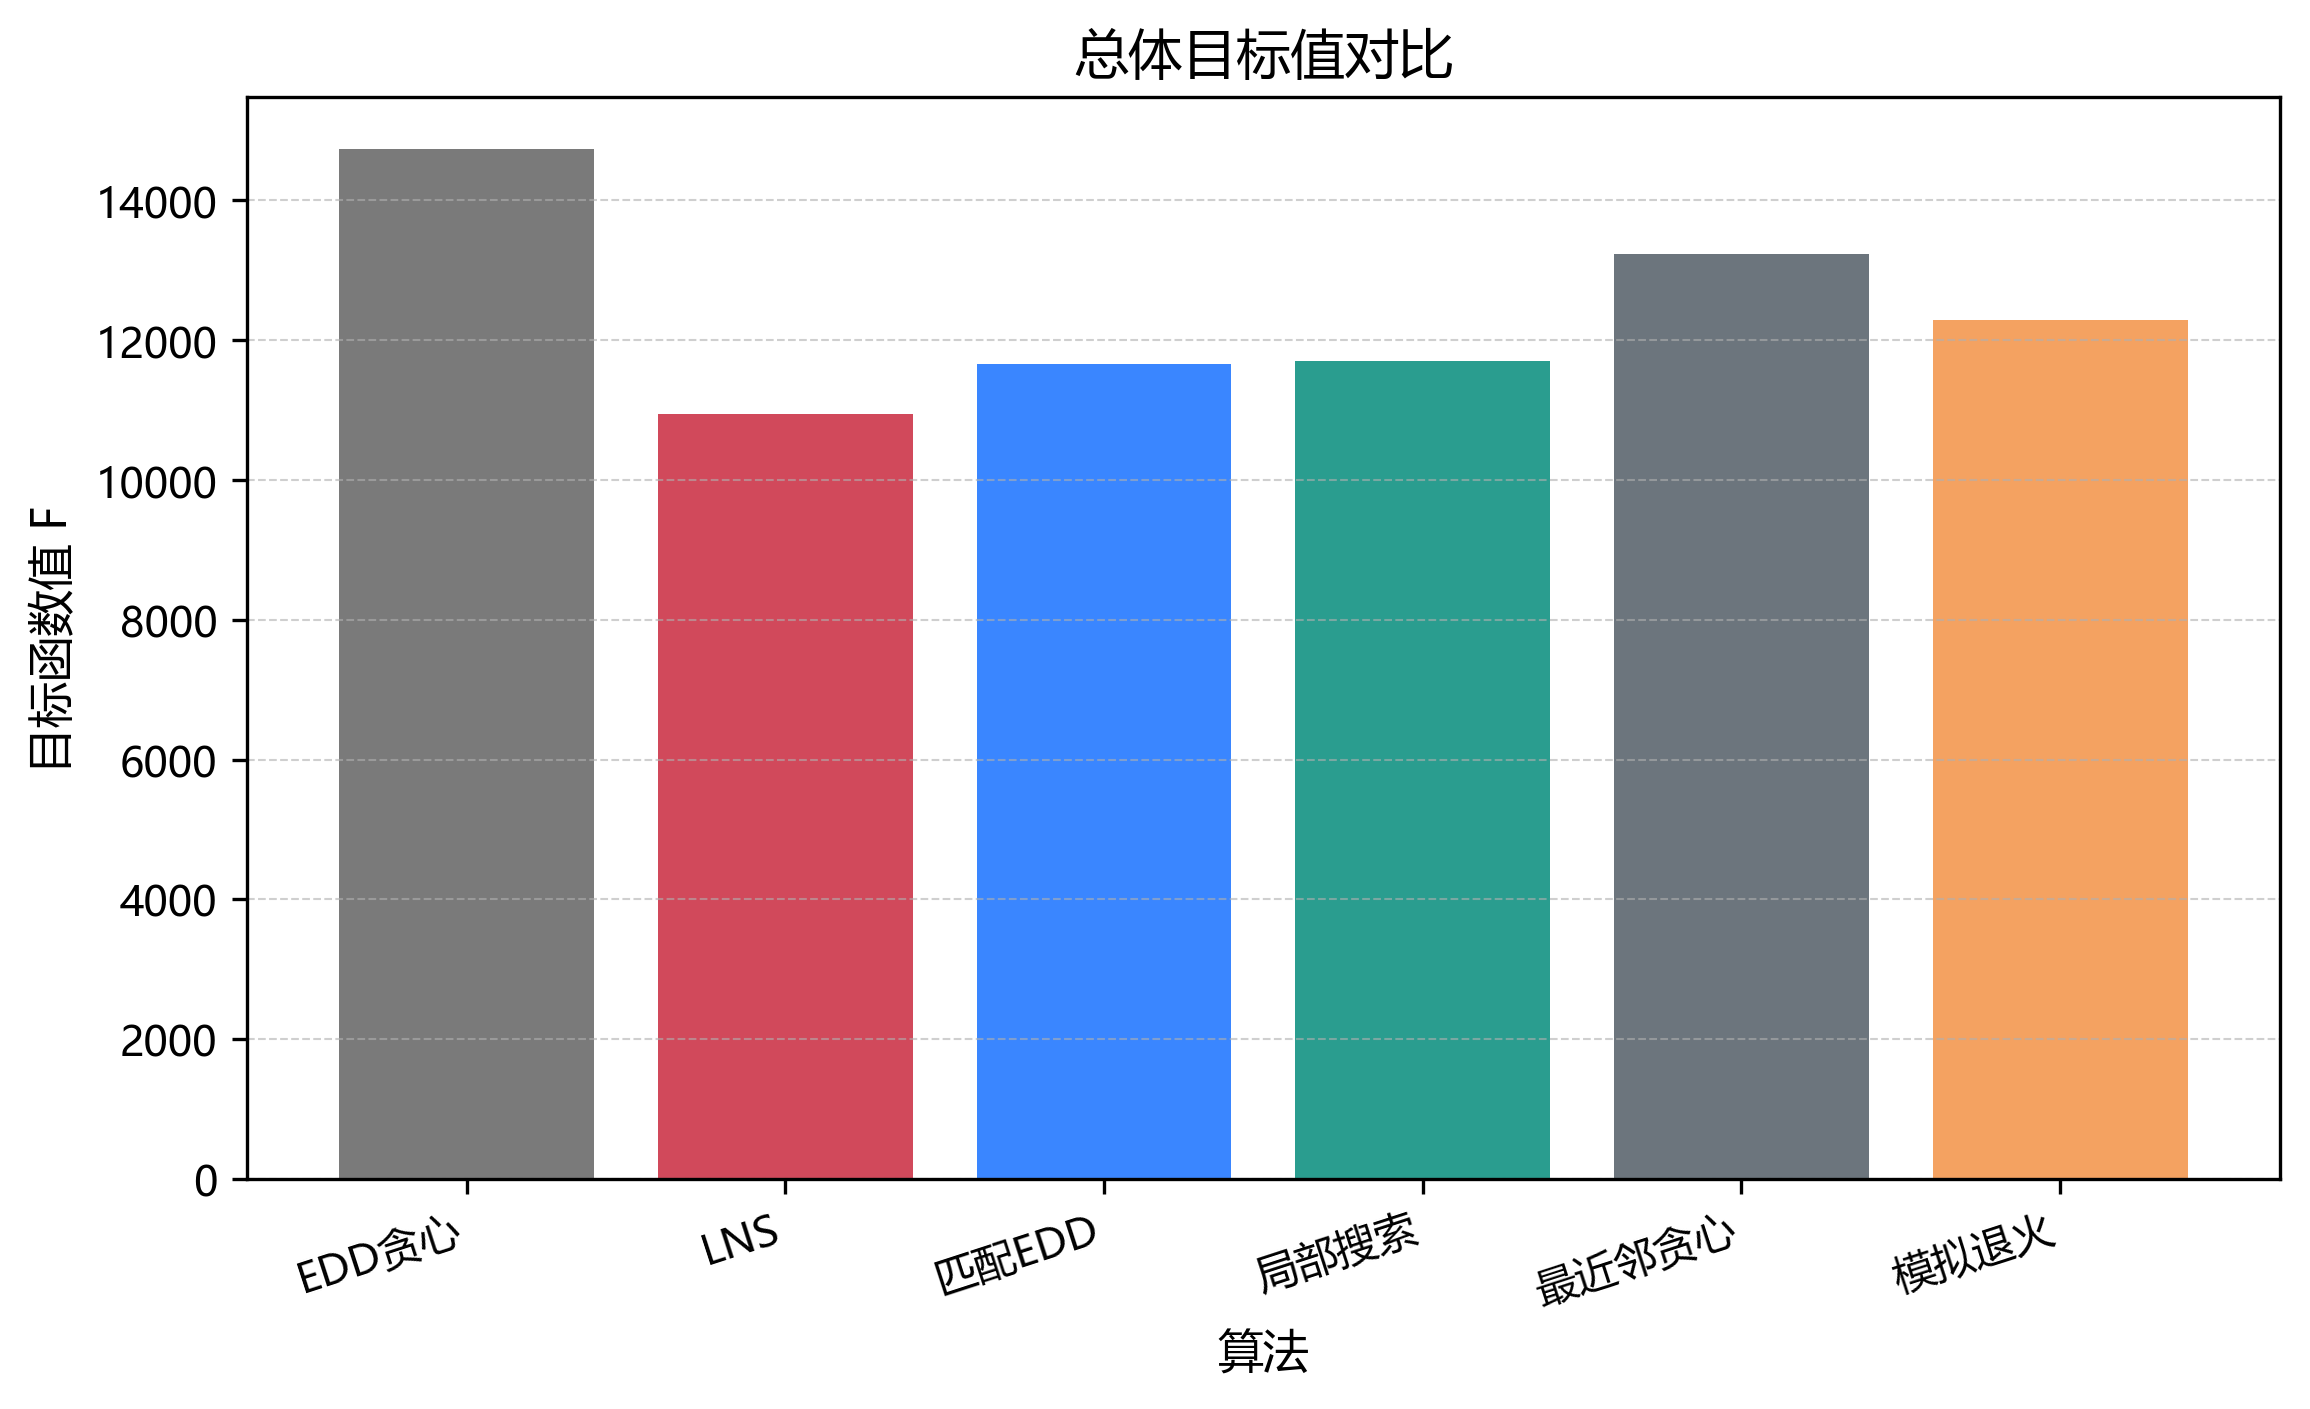
\includegraphics[width=\linewidth]{fig01_overall_objective.png}}
\hfill
\subcaptionbox{总体运行时间\label{fig:overall-time}}[0.48\linewidth]{%
  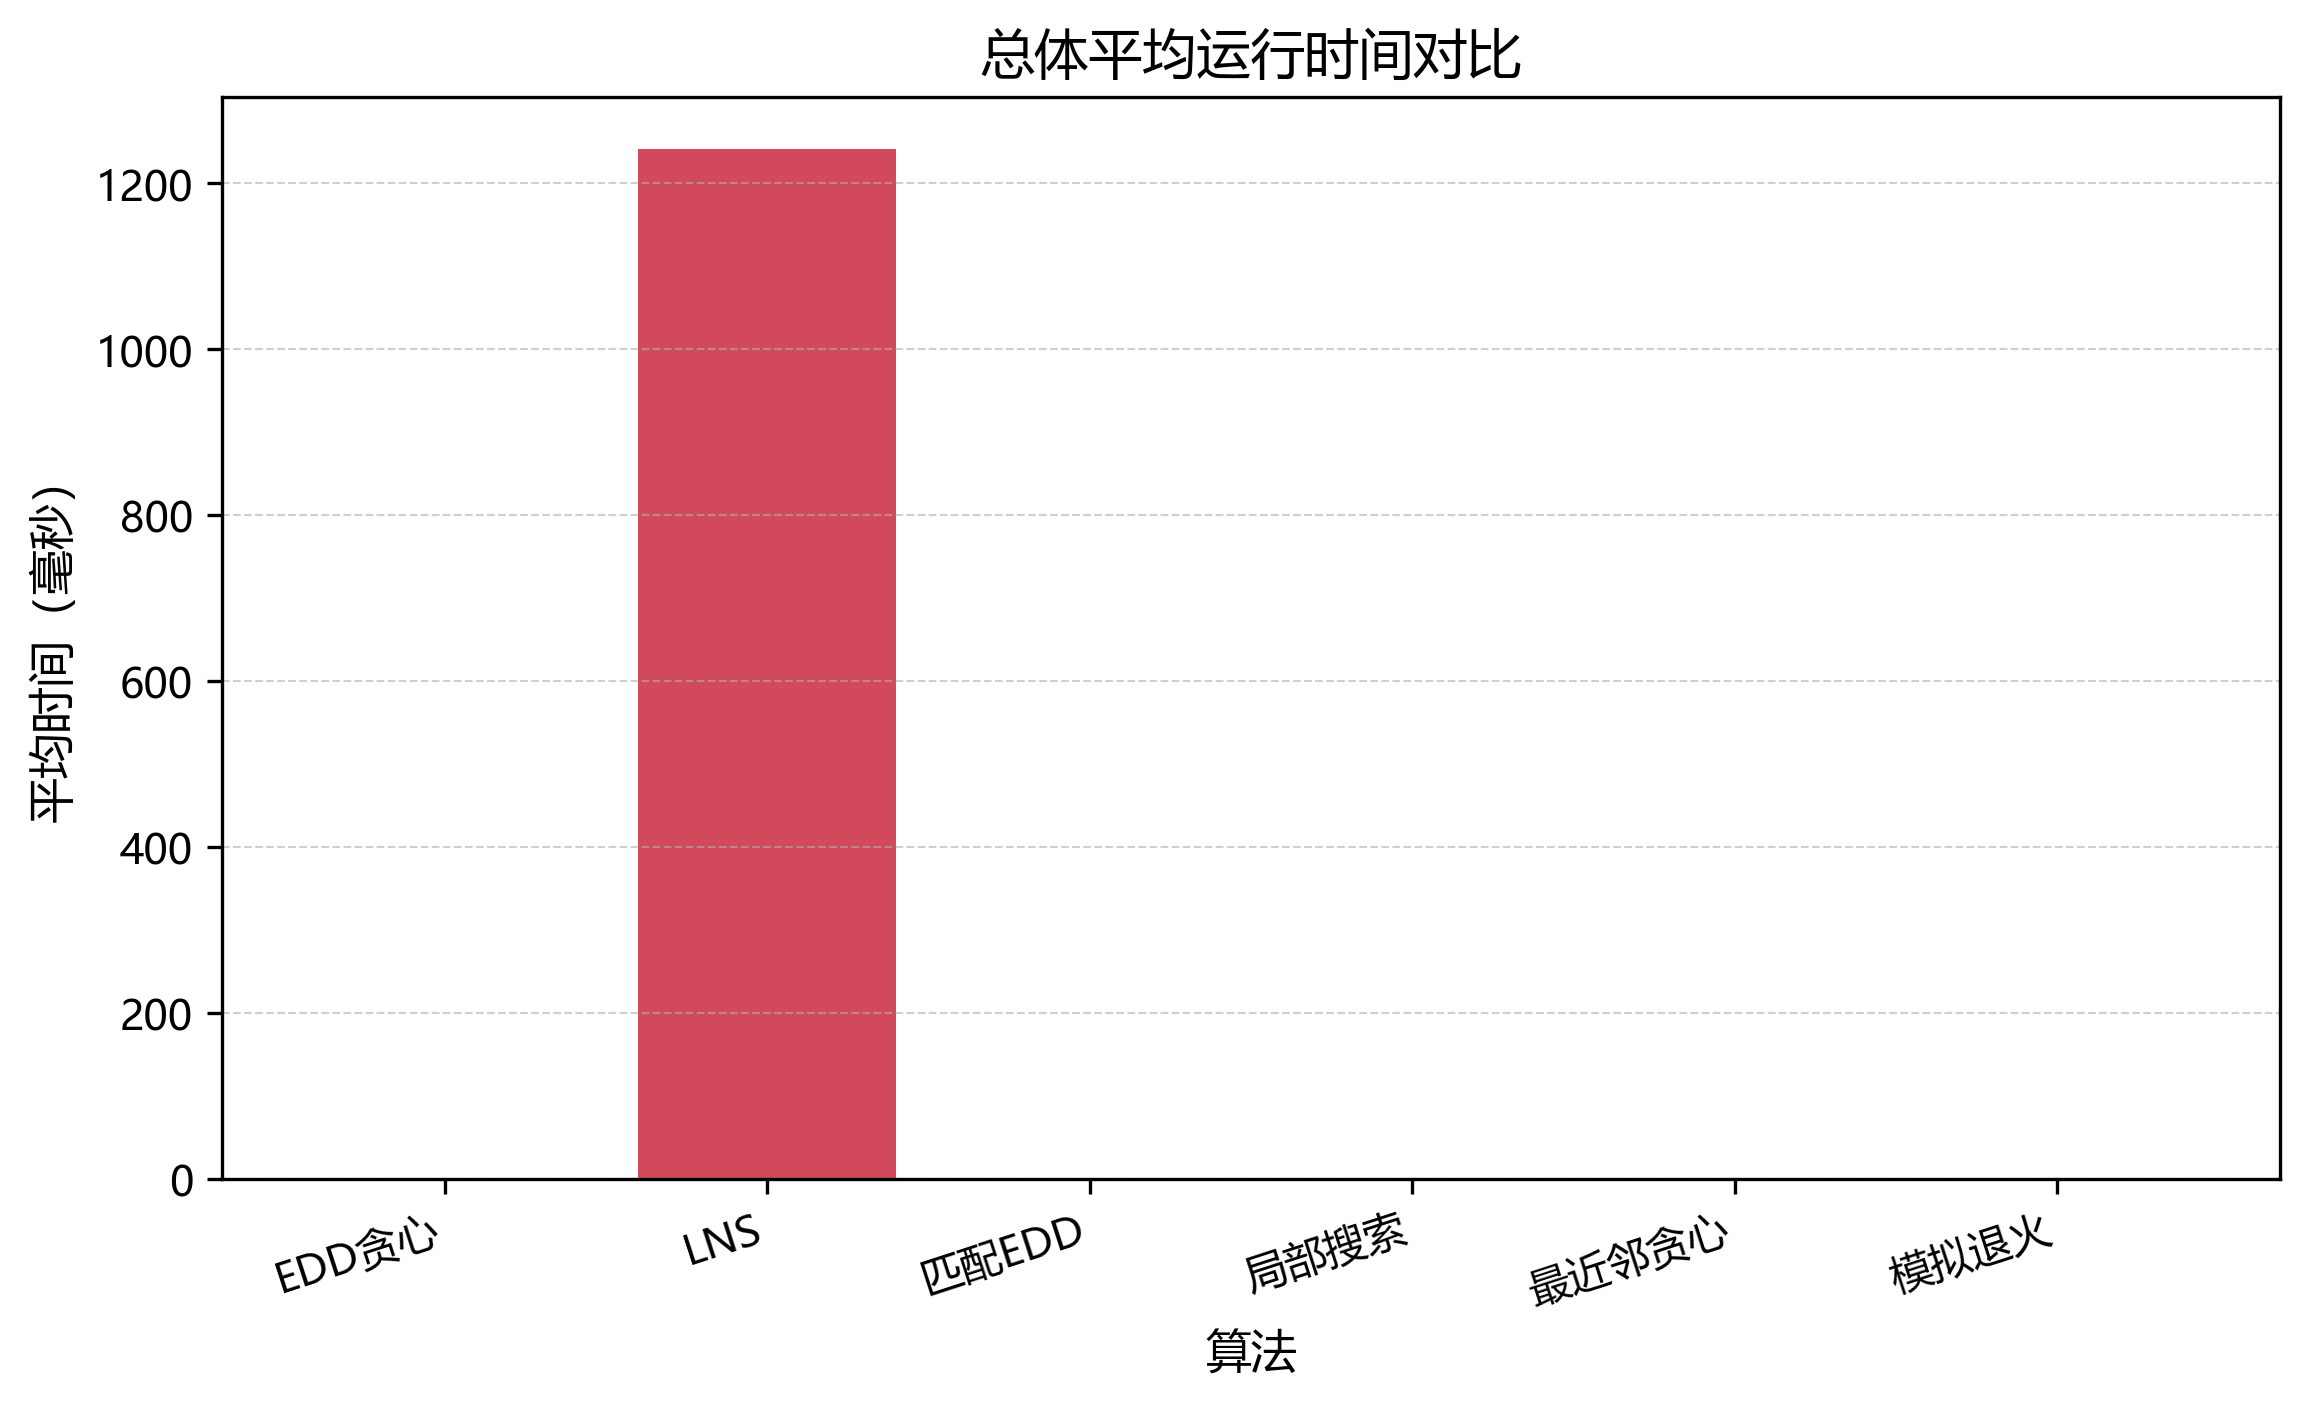
\includegraphics[width=\linewidth]{fig02_overall_runtime.png}}
\caption{主设置下各算法的综合目标值与运行时间比较。}
\end{figure}

\begin{figure}[!tbp]
\centering
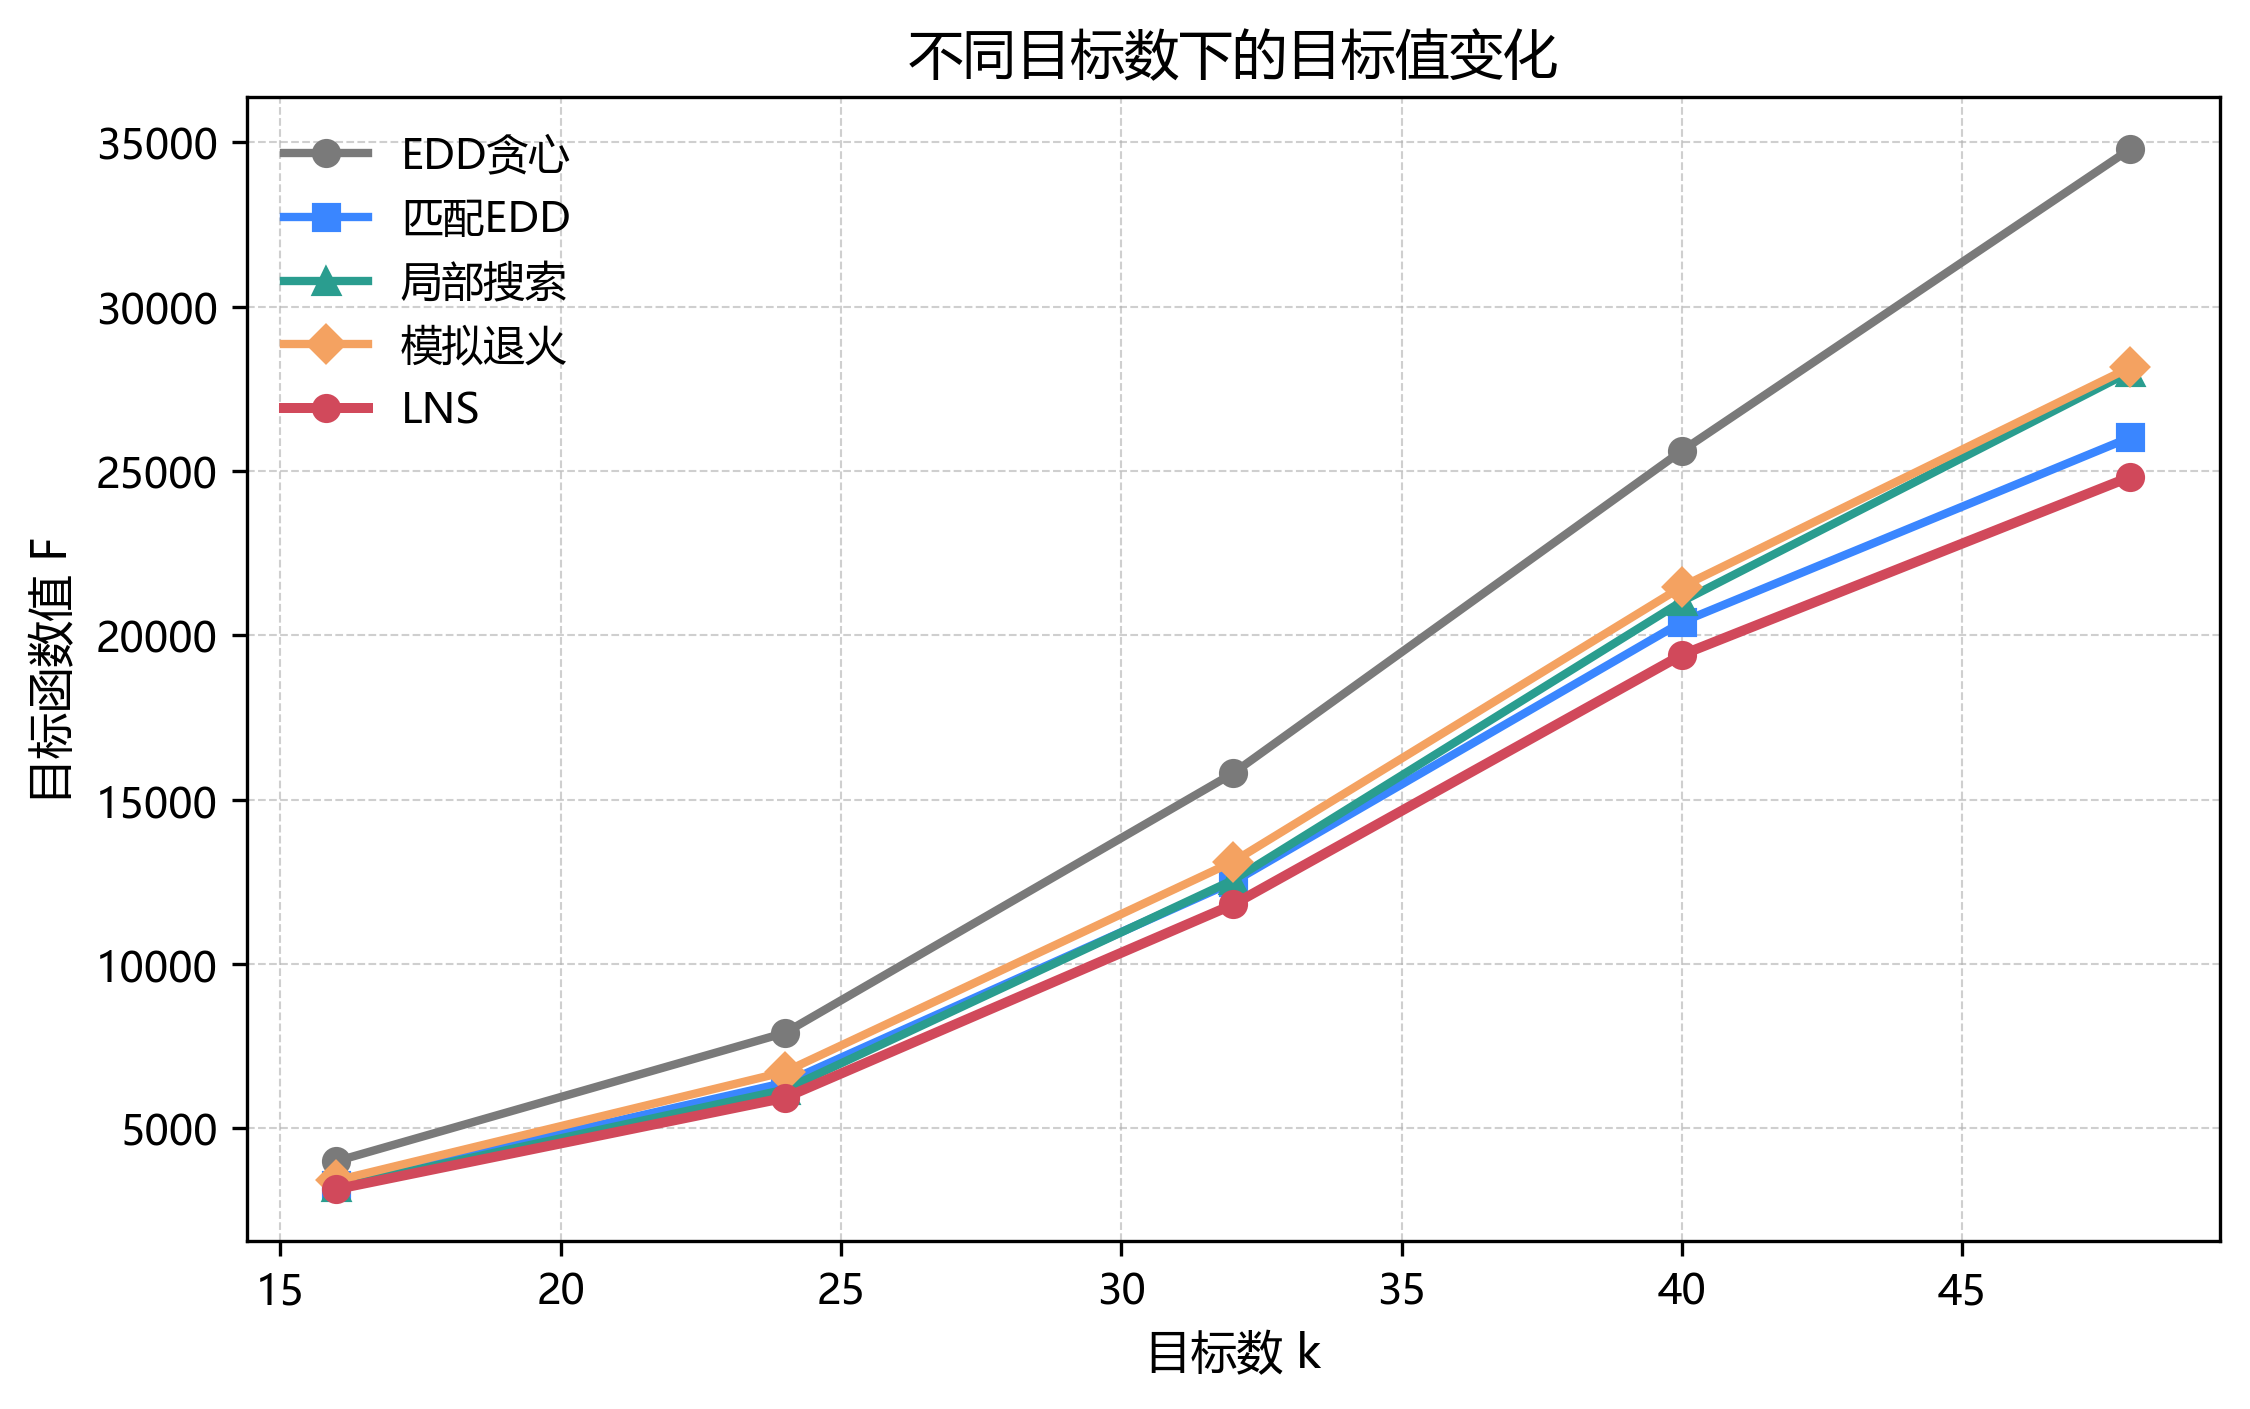
\includegraphics[width=0.92\linewidth]{fig03_objective_by_k.png}
\caption{不同目标数下的目标值变化。}
\label{fig:k-obj}
\end{figure}

\indent 图~\ref{fig:exact} 和图~\ref{fig:gap} 表明，在可穷举的小规模实例上，LNS 与精确最优值接近，明显优于匹配 EDD。模拟退火在小规模下也接近最优，因此 LNS 的主要价值仍体现在较大规模场景。

\begin{figure}[!htbp]
\centering
\subcaptionbox{小规模精确最优值对比\label{fig:exact}}[0.48\linewidth]{%
  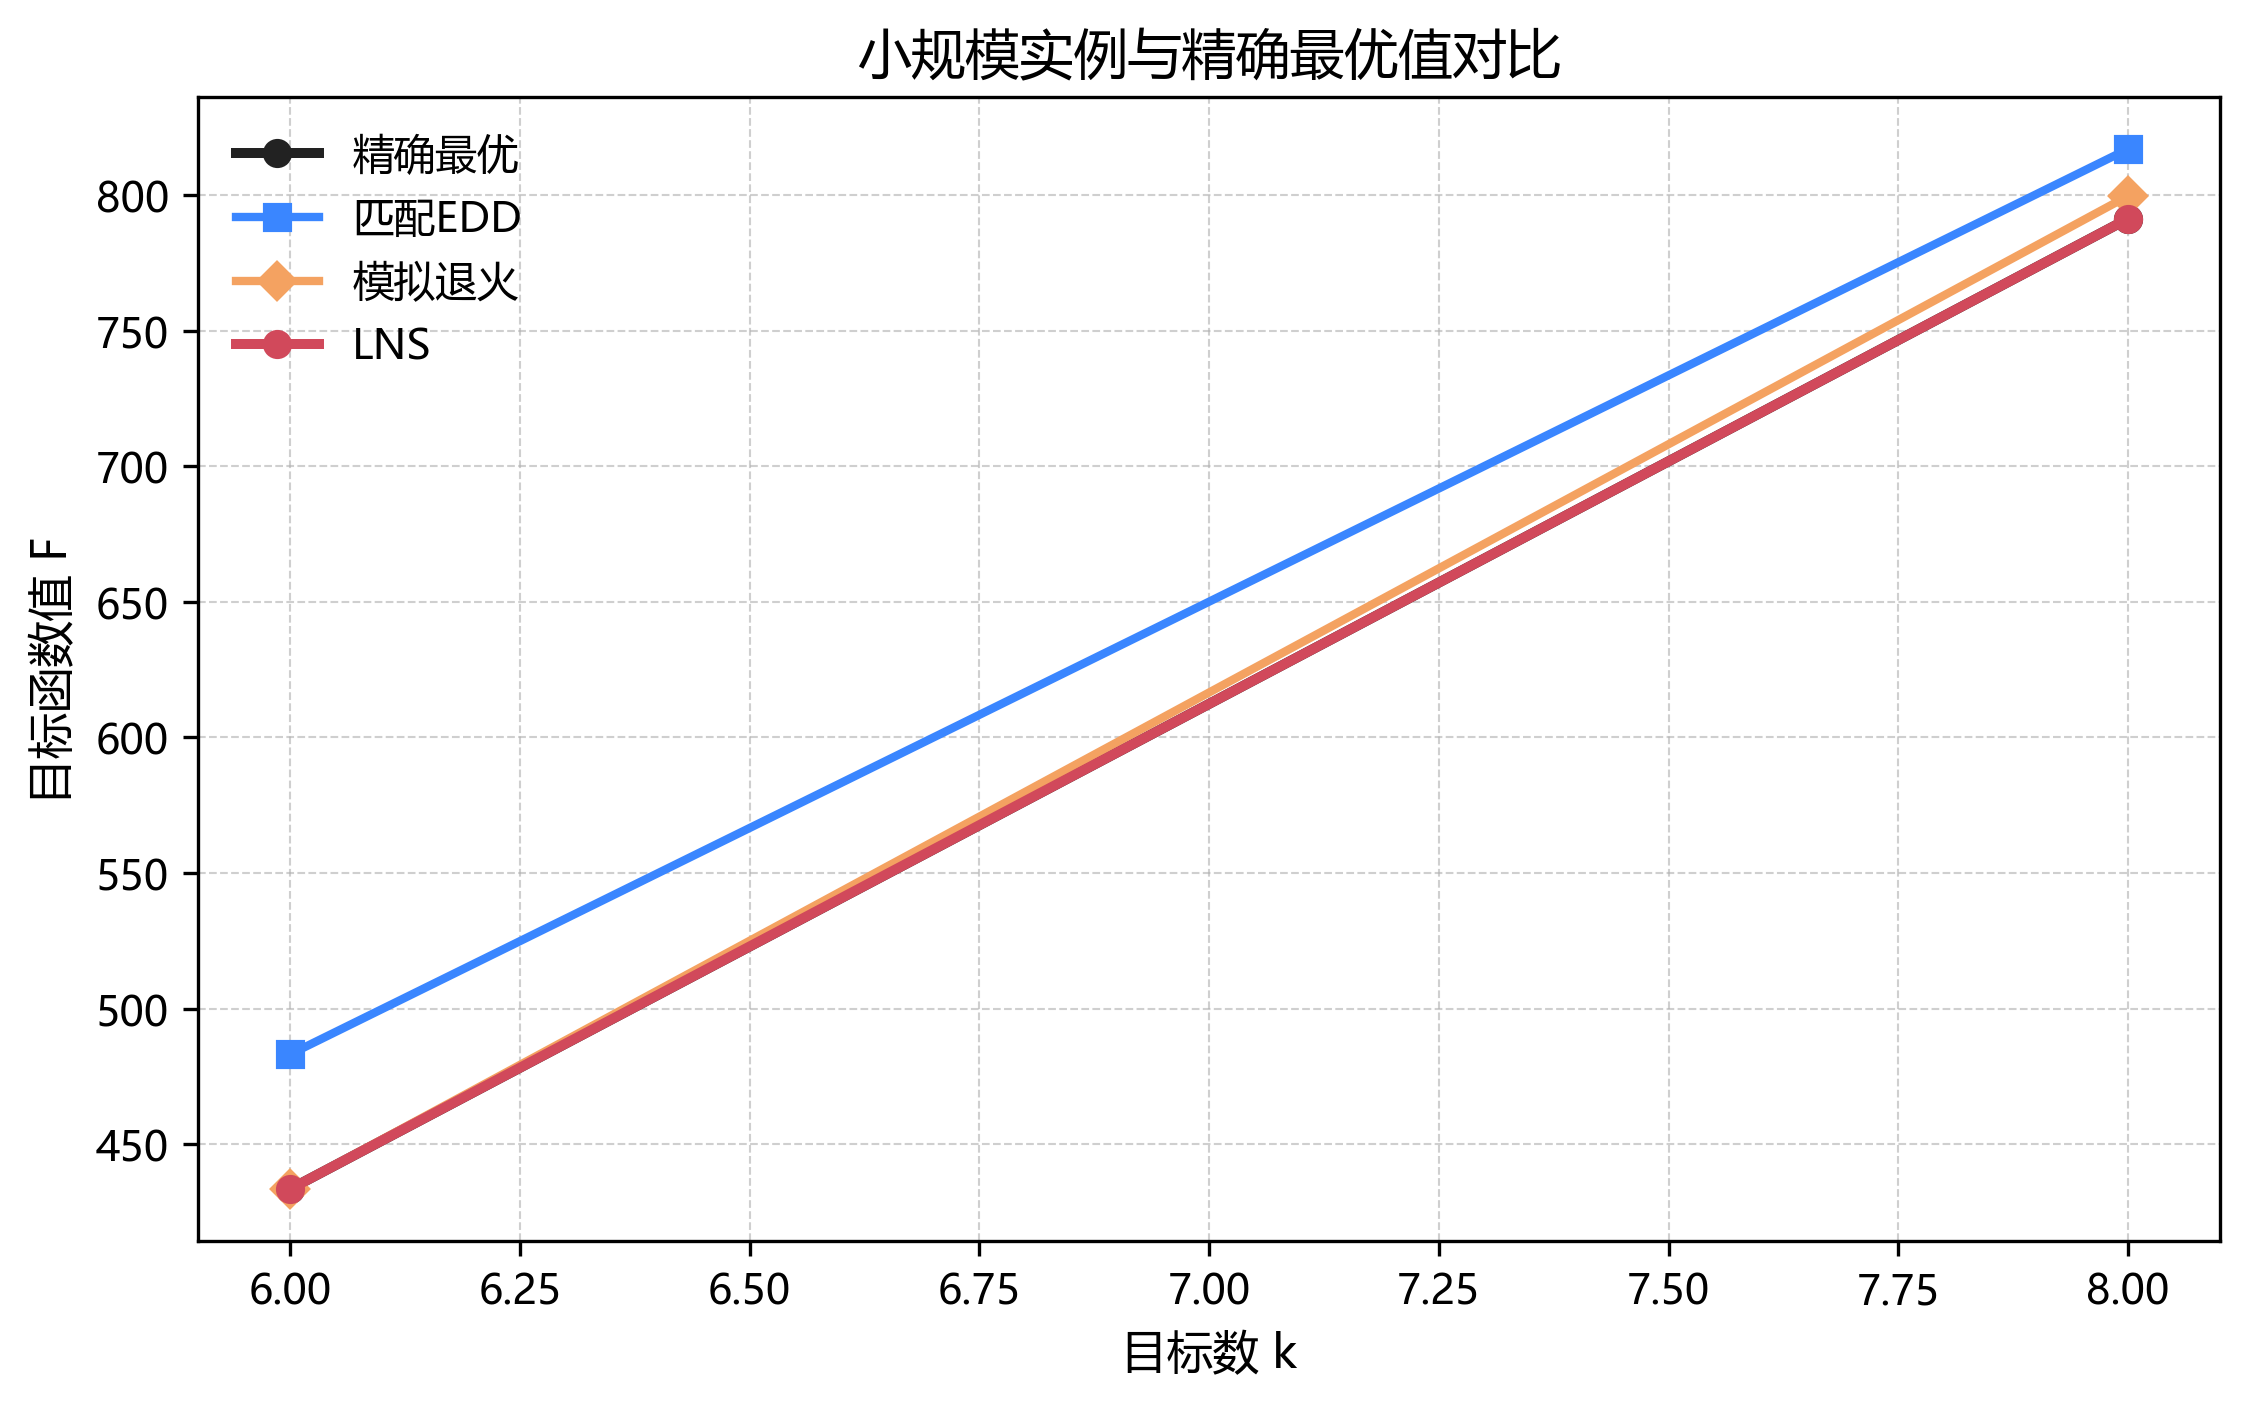
\includegraphics[width=\linewidth]{fig10_exact_optimum_comparison.png}}
\hfill
\subcaptionbox{相对最优差距\label{fig:gap}}[0.48\linewidth]{%
  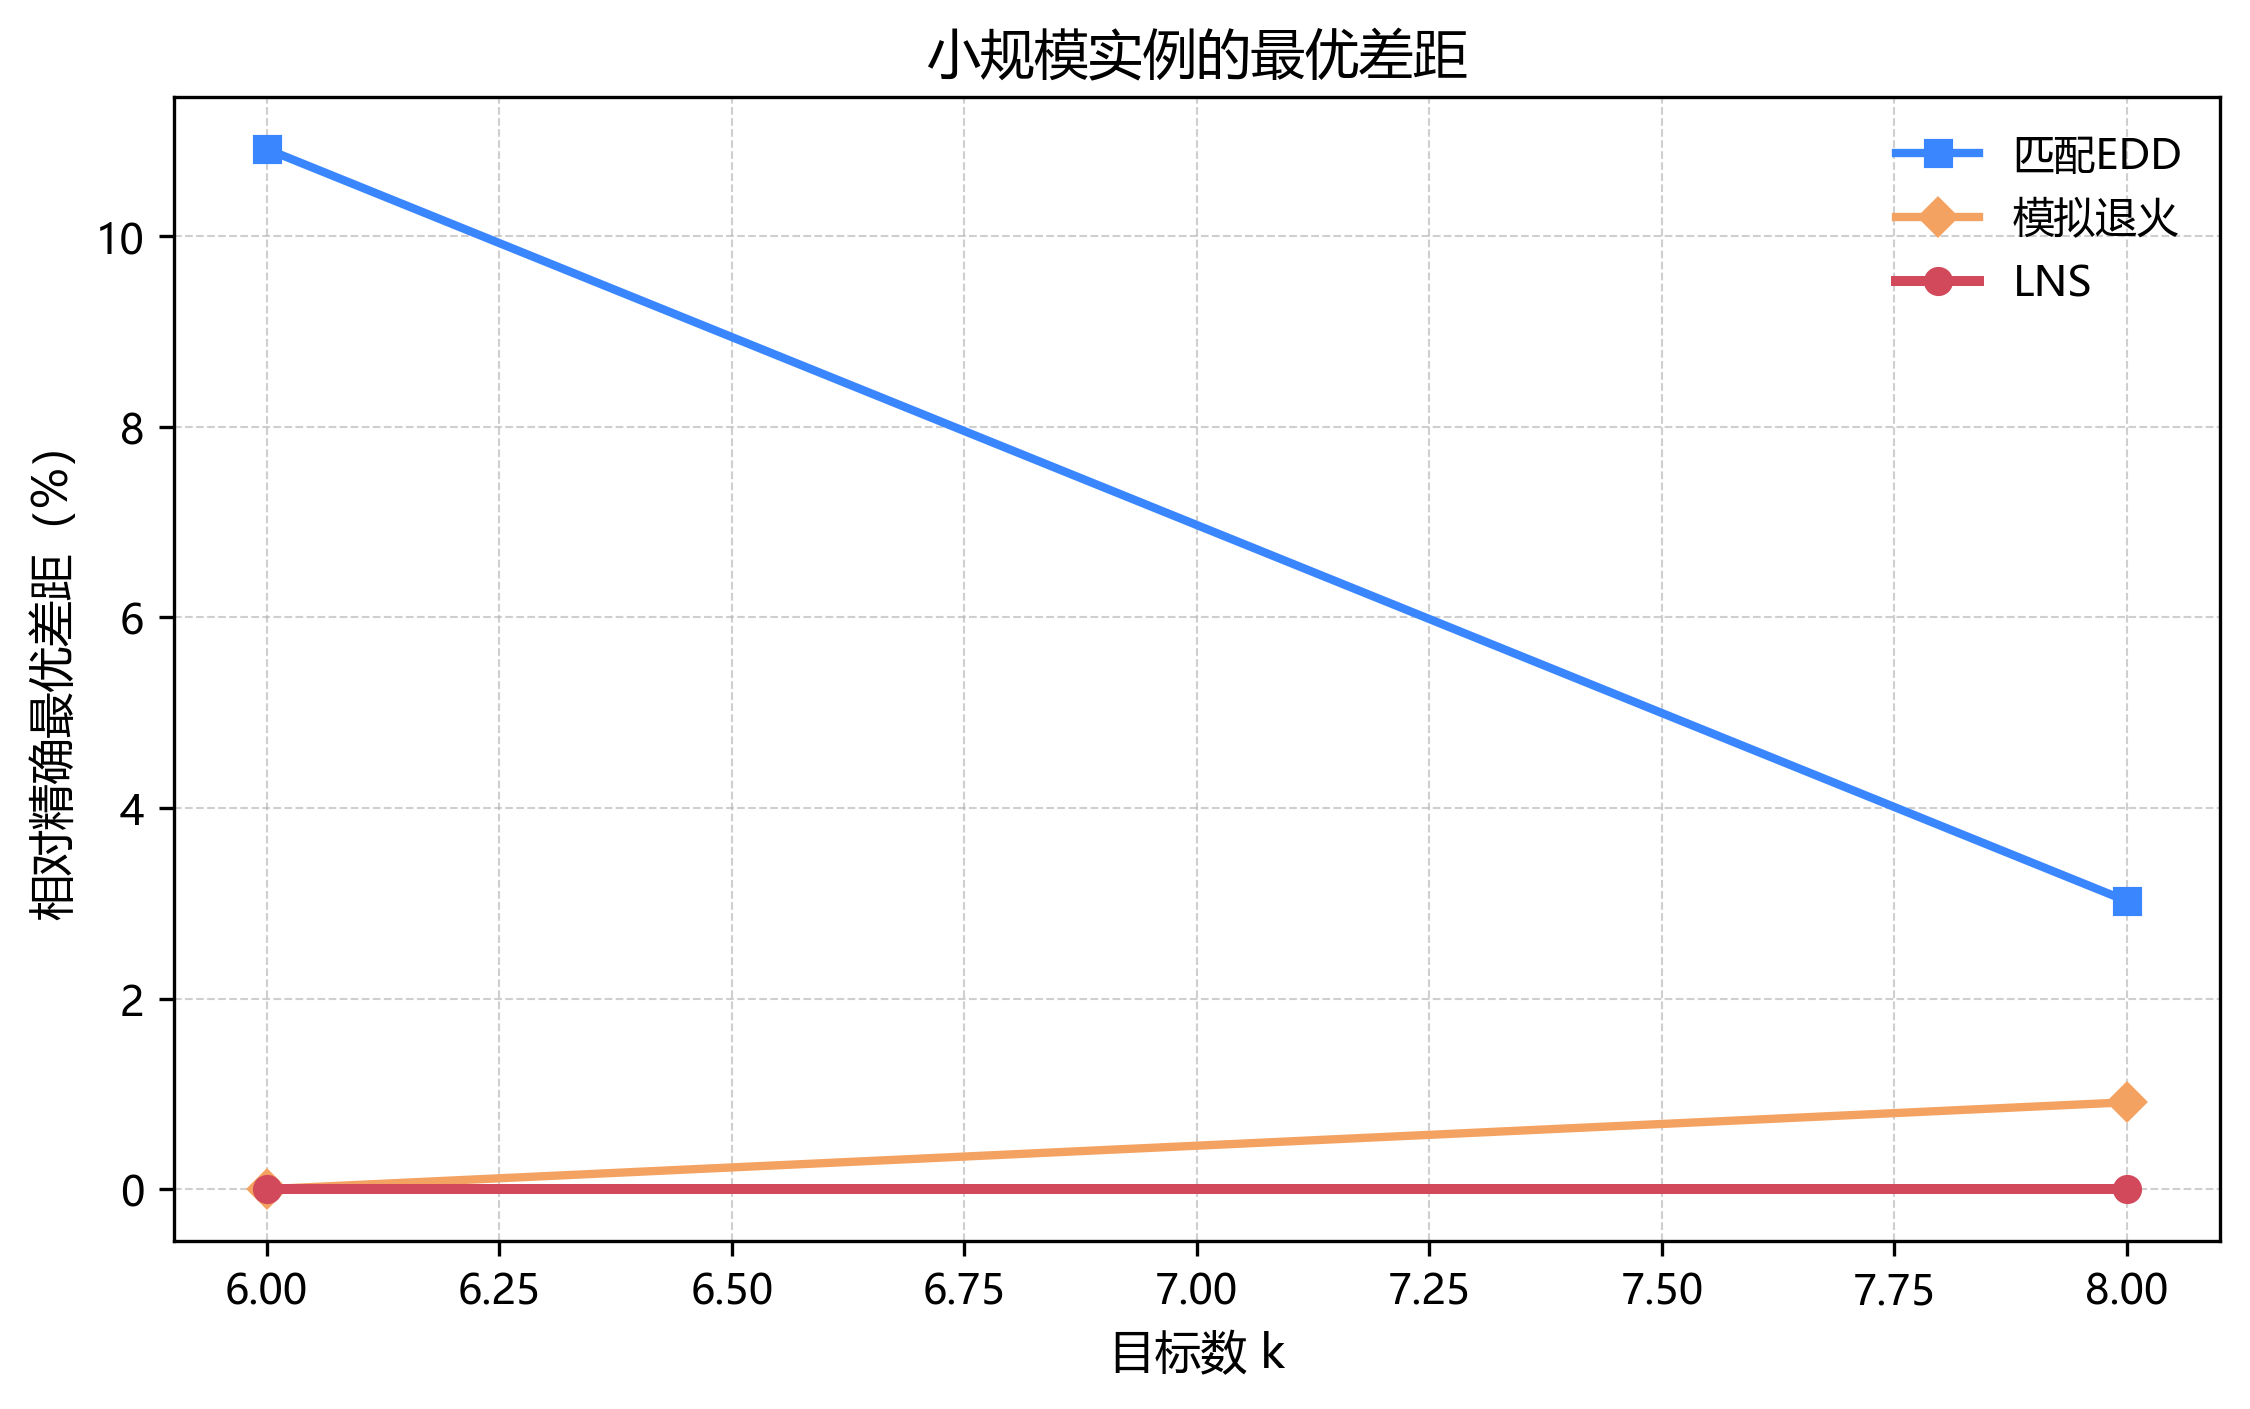
\includegraphics[width=\linewidth]{fig11_optimality_gap_pct.png}}
\caption{小规模实例上的最优性检验。}
\end{figure}

\subsection{统一时间预算与扩展消融}

\indent 图~\ref{fig:budget-meanf} 给出 $300$ ms 统一时间预算下的结果。小规模时 LNS 与模拟退火接近，但当 $k\ge 32$ 后，LNS 明显落后于模拟退火和局部搜索；其平均差距从 $k=32$ 的 $2.32\%$ 上升到 $k=64$ 的 $17.85\%$。这说明短时预算下，LNS 的破坏--修复开销偏大。

\indent 图~\ref{fig:budget-ablation} 给出 $k=32$ 下的扩展消融结果。去除局部强化后平均差距达到 $11.61\%$，说明它是当前实现中最关键的组成部分；去除自适应权重和概率接受也会使结果变差。另一方面，在 $300$ ms 的短预算下，较小破坏比例 $0.15$ 和无后悔插入变体反而接近或优于完整版本，说明短时预算更偏好轻量修复策略。

\begin{figure}[!htbp]
\centering
\subcaptionbox{统一时间预算下不同 $k$ 的平均目标值。\label{fig:budget-meanf}}[0.48\linewidth]{%
  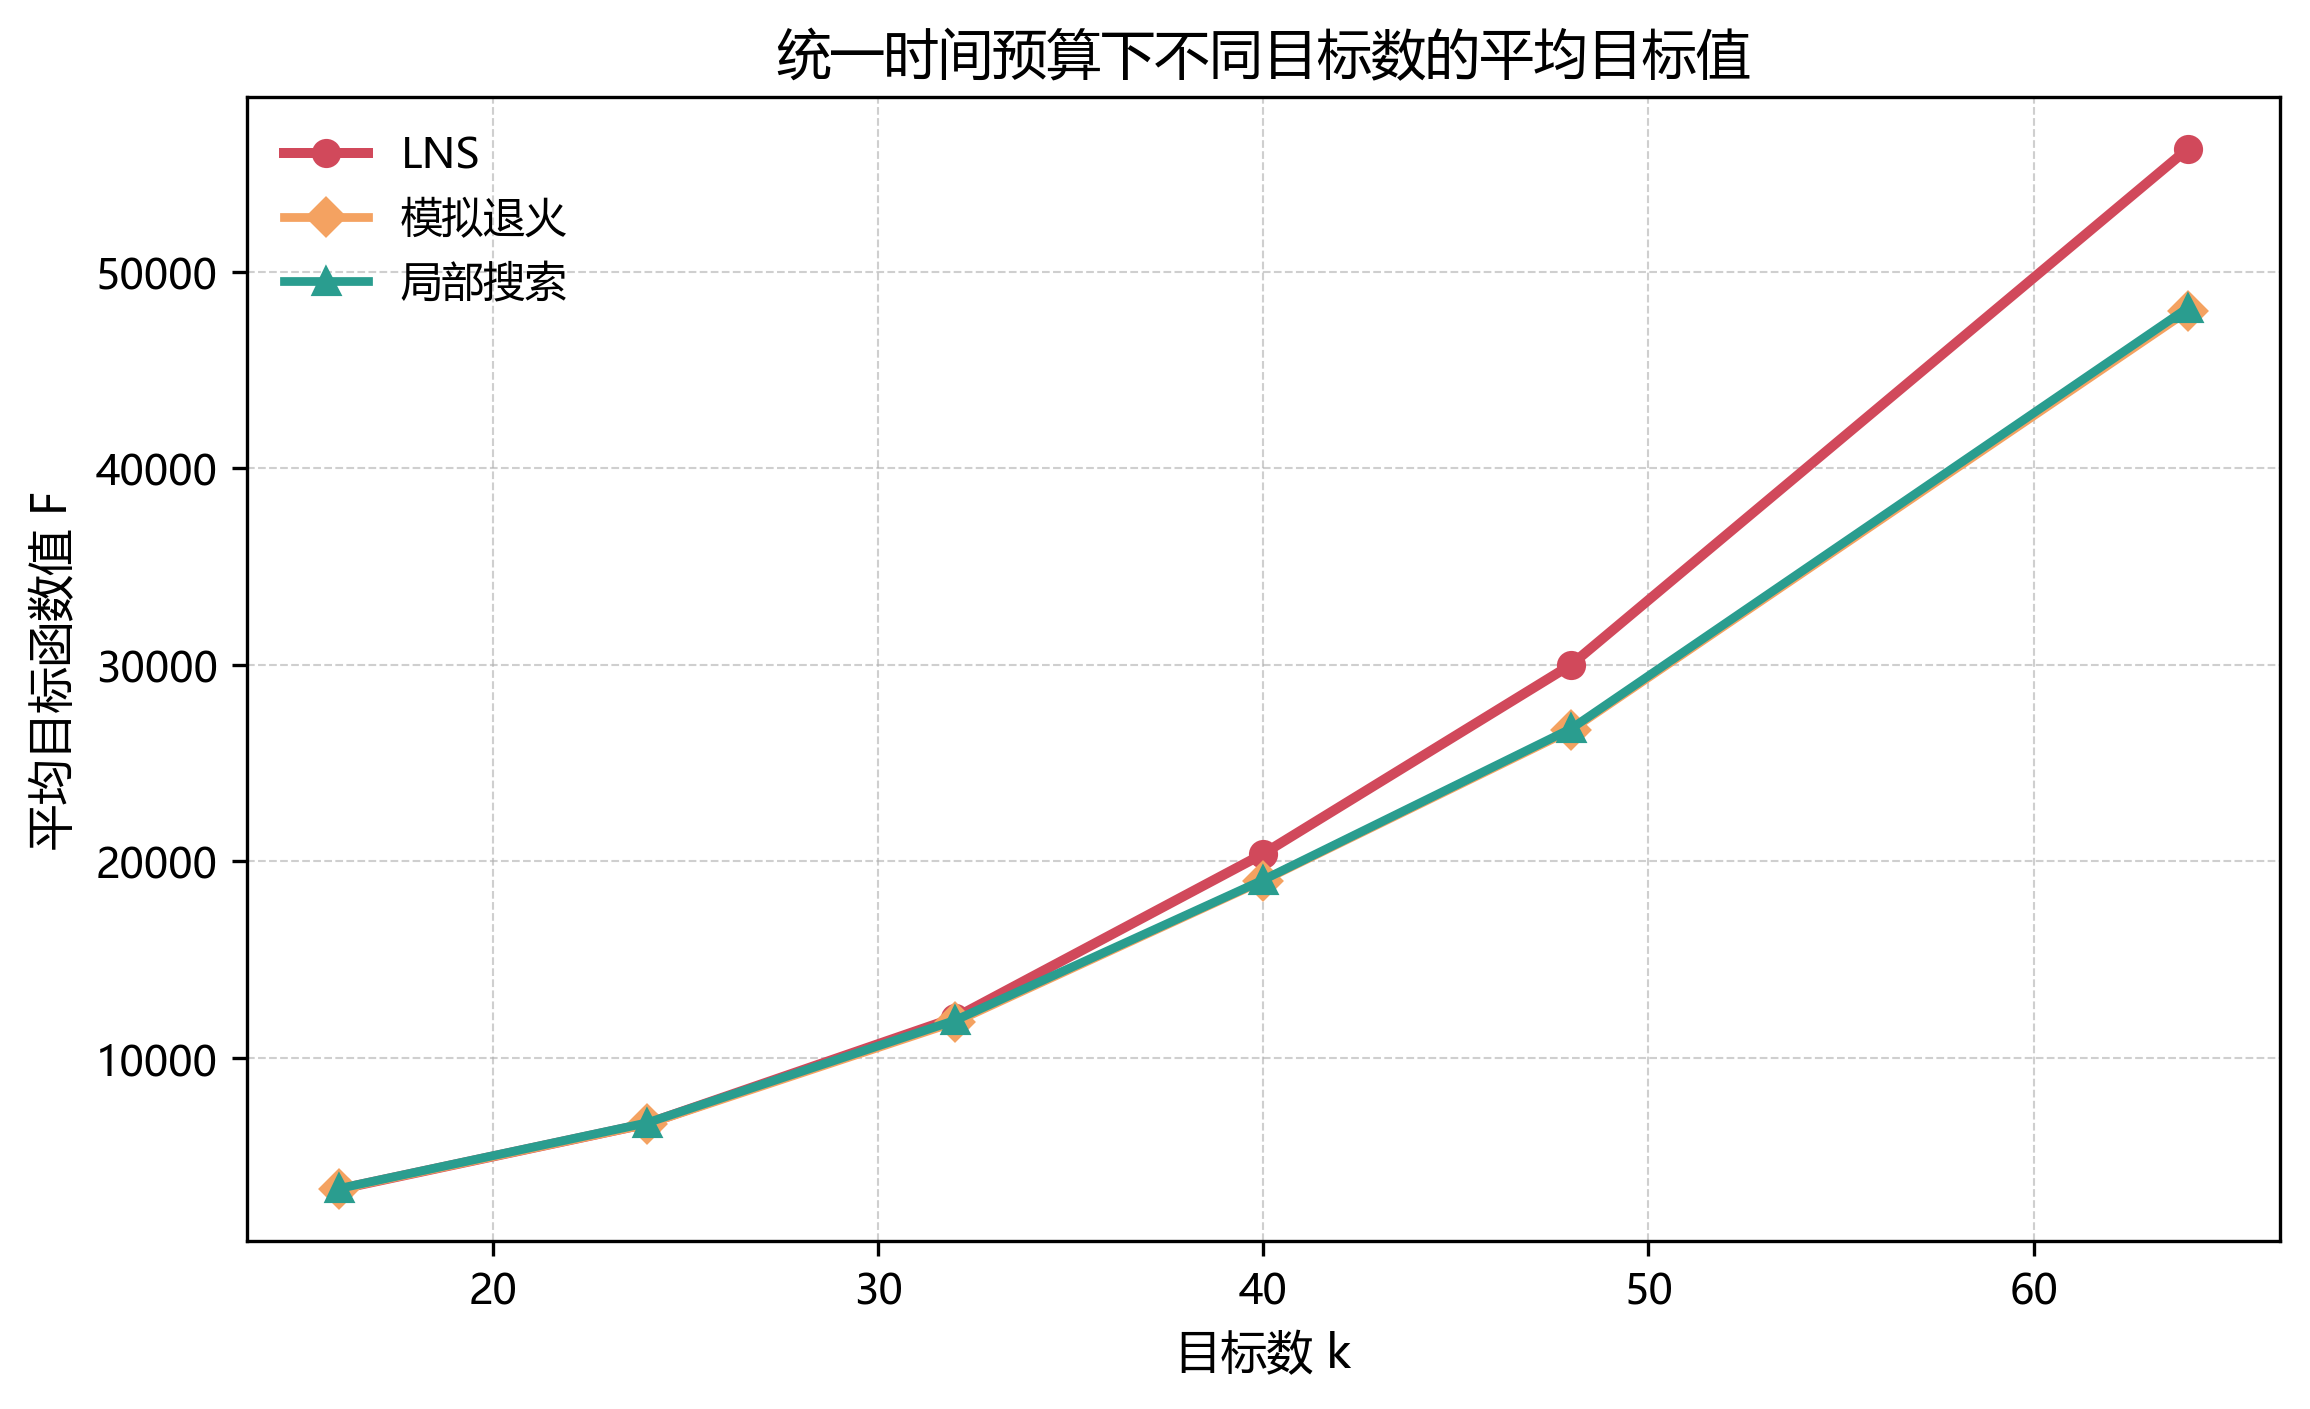
\includegraphics[width=\linewidth]{budget_mean_objective_by_k.png}}
\hfill
\subcaptionbox{$k=32$、$300$ ms 下扩展消融的平均差距。\label{fig:budget-ablation}}[0.48\linewidth]{%
  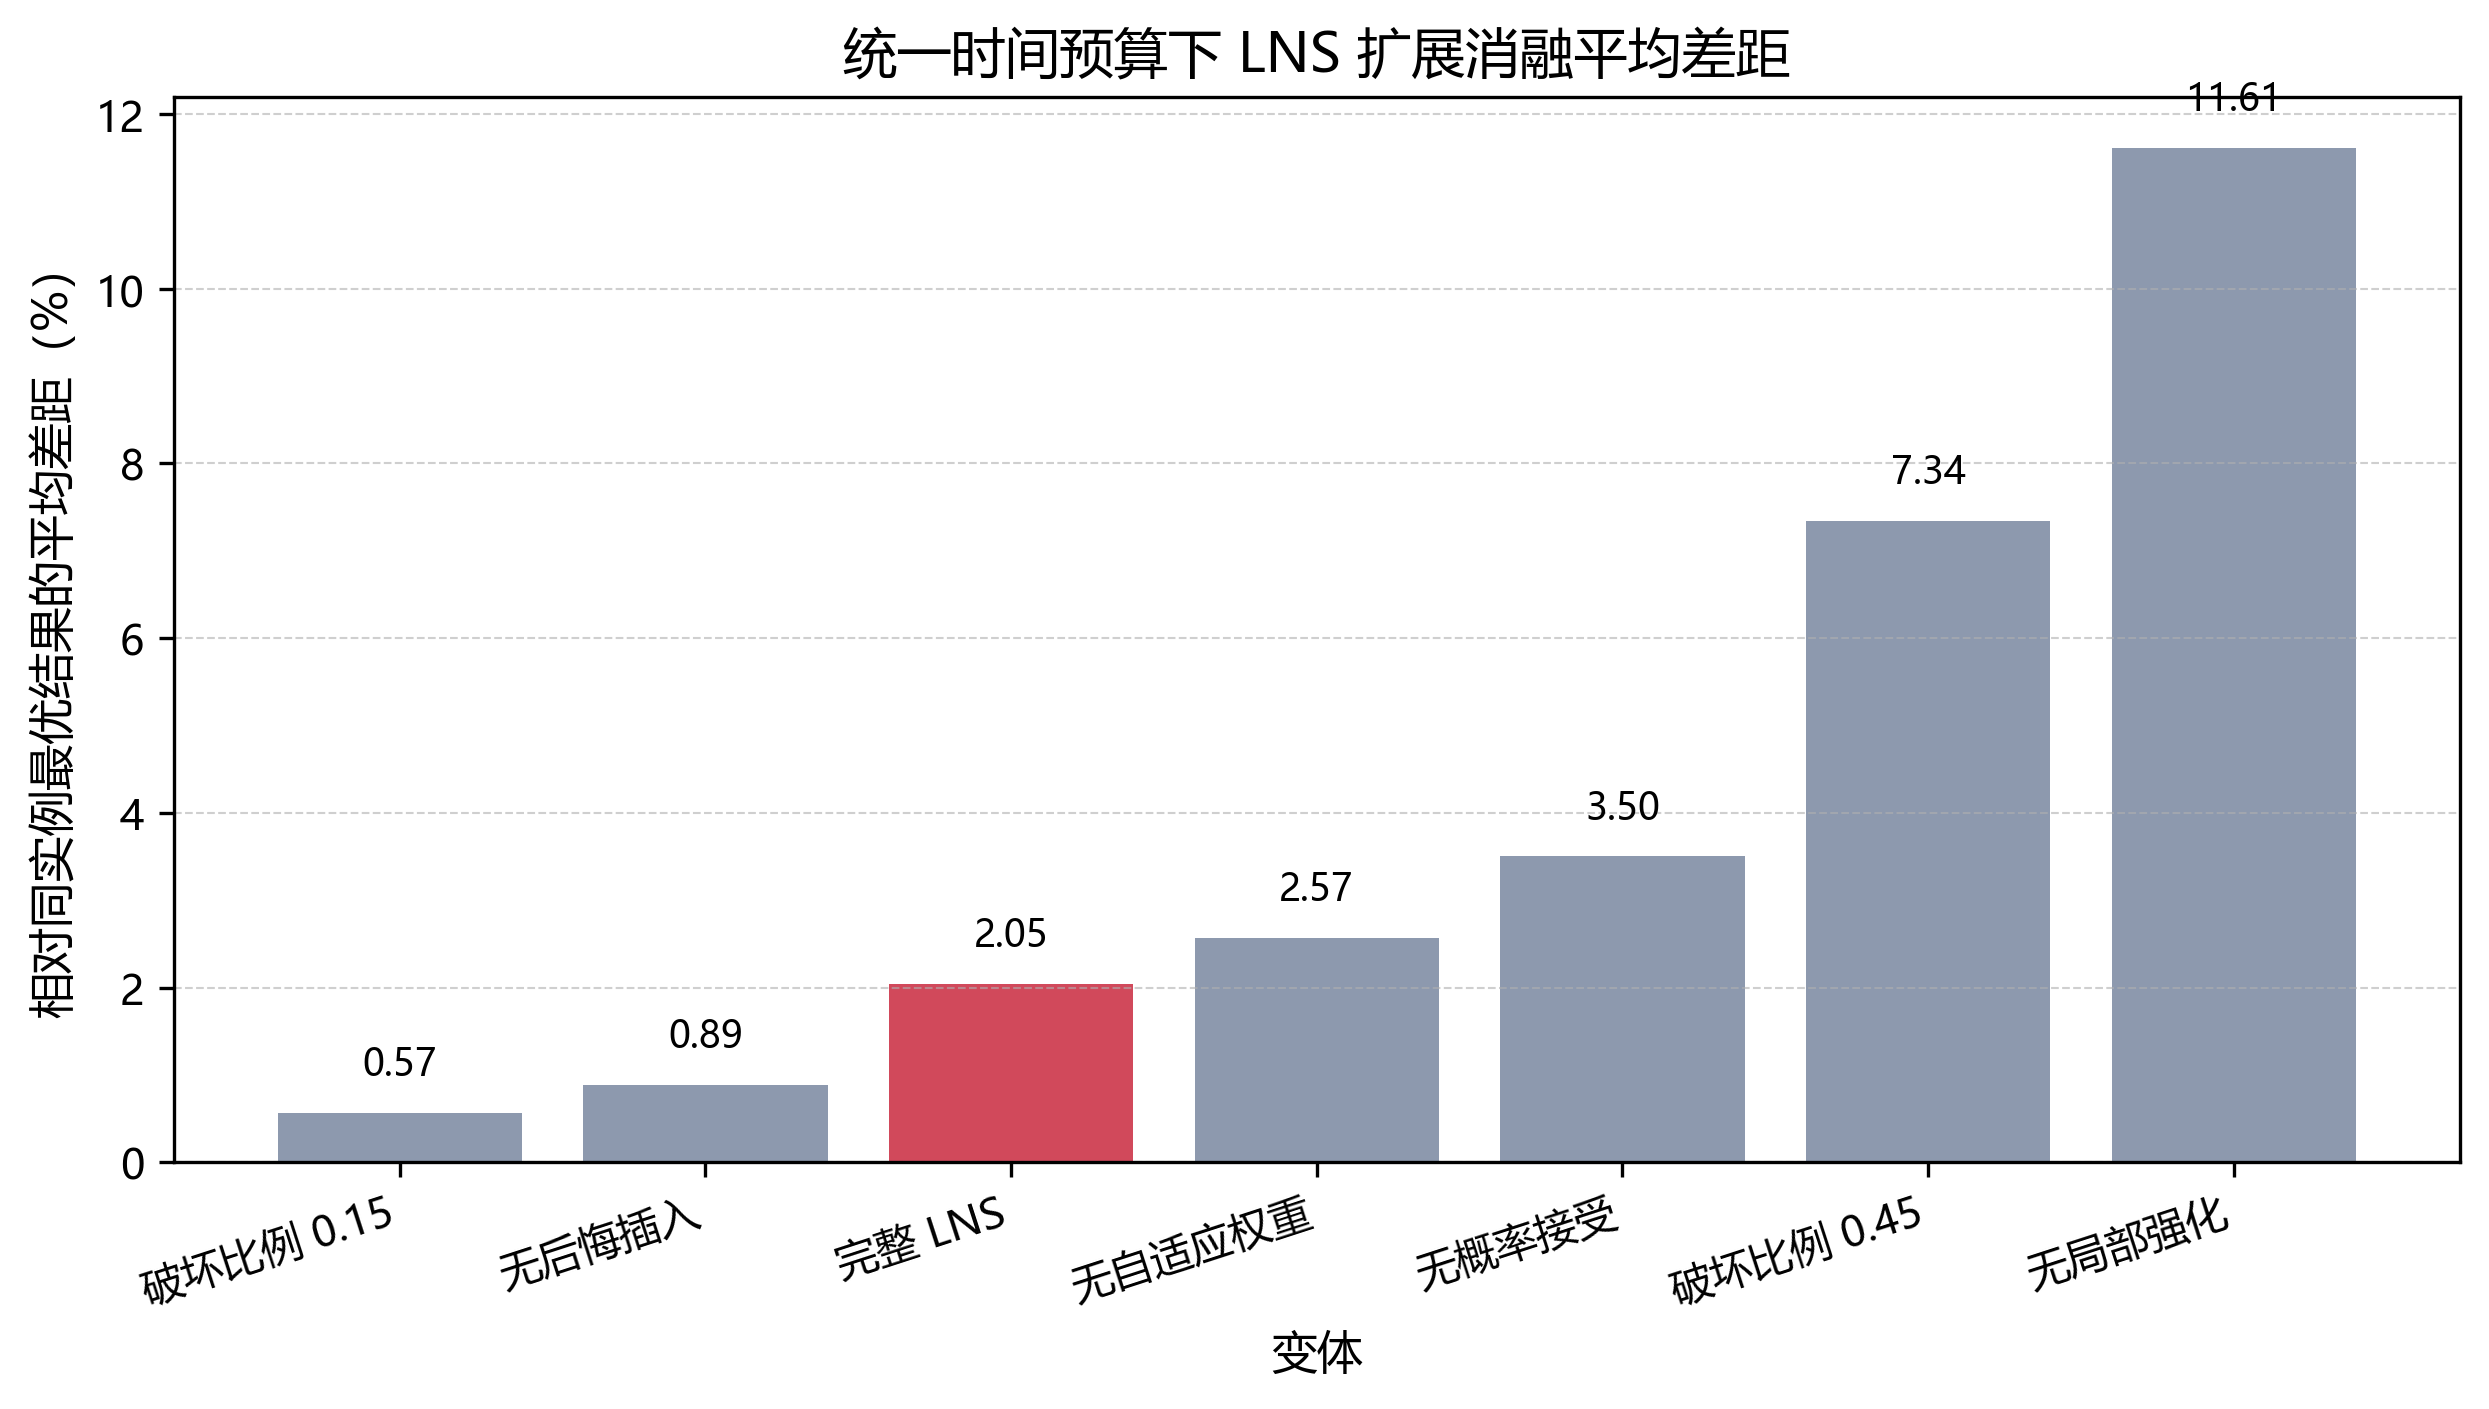
\includegraphics[width=\linewidth]{ablation_k32.png}}
\caption{统一时间预算实验与扩展消融结果。}
\end{figure}

\FloatBarrier

\section{讨论}

\indent 固定迭代预算下，LNS 的优势主要来自较大规模下的结构性重构能力；统一时间预算下，它的主要不足则是修复阶段过重，导致短时 anytime 表现不如模拟退火和局部搜索。因此，若强调快速响应，更适合选用模拟退火或局部搜索；若强调解质量且允许更长计算时间，LNS 更有价值。

\indent 本文实验仍基于随机网格实例。后续可进一步引入真实或半真实地图、动态订单、多个配送员和更多预算点，以检验该框架在更接近实际场景下的表现。

\section{结论}

\indent 本文研究了带时间惩罚的双载荷网格配送问题，并提出基于有序配对排列的 LNS 方法。实验表明：在固定迭代预算下，LNS 往往能取得更低目标值；在统一 $300$ ms 时间预算下，LNS 因重构开销较大而不占优。因此，更合适的定位是把 LNS 视为较长预算下的高质量启发式框架，而不是所有预算下都占优的通用方法。后续可继续从增量评价、预算自适应策略和更真实的数据集三个方向改进。

\begin{thebibliography}{99}
\bibitem{shaw1998}
Shaw P. Using constraint programming and local search methods to solve vehicle routing problems. In: \emph{Proceedings of the 4th International Conference on Principles and Practice of Constraint Programming}, 1998: 417--431.

\bibitem{ropke2006}
Ropke S., Pisinger D. An adaptive large neighborhood search heuristic for the pickup and delivery problem with time windows. \emph{Transportation Science}, 2006, 40(4): 455--472.

\bibitem{kirkpatrick1983}
Kirkpatrick S., Gelatt C. D., Vecchi M. P. Optimization by simulated annealing. \emph{Science}, 1983, 220(4598): 671--680.

\bibitem{pisinger2010}
Pisinger D., Ropke S. Large neighborhood search. In: Gendreau M., Potvin J.-Y. (eds.) \emph{Handbook of Metaheuristics}. 2nd ed. Boston: Springer, 2010: 399--419.

\bibitem{solomon1987}
Solomon M. M. Algorithms for the vehicle routing and scheduling problems with time window constraints. \emph{Operations Research}, 1987, 35(2): 254--265.

\bibitem{laporte1992}
Laporte G. The vehicle routing problem: An overview of exact and approximate algorithms. \emph{European Journal of Operational Research}, 1992, 59(3): 345--358.

\bibitem{cormen2009}
Cormen T. H., Leiserson C. E., Rivest R. L., Stein C. \emph{Introduction to Algorithms}. 3rd ed. Cambridge, MA: MIT Press, 2009.

\bibitem{toth2014}
Toth P., Vigo D. (eds.) \emph{Vehicle Routing: Problems, Methods, and Applications}. 2nd ed. Philadelphia: SIAM, 2014.
\end{thebibliography}

\end{document}
